%%%%%%%%%%%%%%%%%%%%%%%%%%%%%%%%%%%%%%%%%%%%%%%%
% Conectividade em florestas dinamicas         %
%%%%%%%%%%%%%%%%%%%%%%%%%%%%%%%%%%%%%%%%%%%%%%%%
\chapter{Conexidade em florestas dinâmicas}
\label{sec:connDF}

O problema de conexidade em grafos dinâmicos, descrito na Seção \ref{sec:Motivação}, pode ser reduzido ao caso em que o grafo é uma floresta, originando assim o \defi[problema!de conexidade em florestas dinâmicas]{problema de conexidade em florestas dinâmicas}. Detalharemos como essa redução é feita no Capítulo~\ref{sec:connDG}. Esse problema pode ser apresentado como a implementação da seguinte biblioteca da forma mais eficiente possível: 

\begin{itemize}
\item \dymForestCreate($n$): cria uma floresta dinâmica com $n$ vértices isolados;
\item \dymForestAddEdge($F$, $u$, $v$): adiciona a aresta $uv$ à floresta dinâmica~$F$;
\item \dymForestDelEdge($F$, $u$, $v$): remove a aresta $uv$ de $F$; e
\item \dymForestQuery($F$, $u$, $v$): retorna verdadeiro se $u$ e $v$ estão na mesma componente conexa de $F$ e falso, caso contrário.
\end{itemize}
 
Há na literatura uma estrutura de dados bem conhecida chamada \defi{link-cut trees} \cite{SleatroTarjanLinkCutTree1983} que resolve uma versão direcionada desse problema, em que as árvores da floresta são enraizadas. Com essa estrutura de dados e uma rotina adicional, que permite mudar a raiz de uma dada árvore para um de seus outros nós, as link-cut trees resolvem também a versão não direcionada do problema, ou seja, o problema de conexidade em florestas dinâmicas. Nessa seção apresentaremos as \defi{Euler tour trees}, uma solução mais simples e tão eficiente quanto.


\section{Euler tour trees} 

Tarjan e Vishkin~\cite{tarjan1985} propuseram a \defi{representação por trilha Euleriana} de uma árvore (originalmente nomeada \textit{Euler tour technique}).
Essa representação é obtida de uma árvore~$T$ substituindo-se cada aresta por dois arcos em sentidos opostos e adicionando-se um laço a cada vértice, como pode ser visto na Figura~\ref{fig:exemploSeqEuler}. O digrafo resultante é \defi{Euleriano}, ou seja, é conexo e possui uma trilha que começa e termina num mesmo vértice e que passa por todos os arcos do digrafo exatamente uma vez. Uma tal trilha é chamada de \defi{trilha Euleriana} do digrafo.


\begin{figure}[htb]
\centering
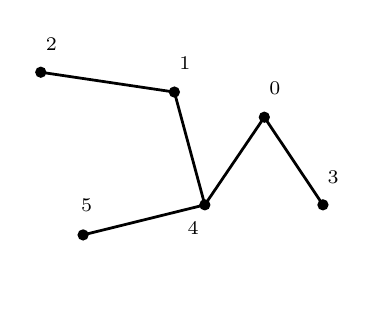
\begin{tikzpicture}[dot/.style={draw,circle,fill,inner sep=1.5pt},line width=1pt,x=1.5cm,y=1.5cm]
\clip(.5,1.3) rectangle (3.3,3.5);
\draw [line width=1pt] (1.7420645075484014,2.9548225063123694)-- (0.6109449986613309,3.1228105521866865);
\draw [line width=1pt] (1.7420645075484014,2.9548225063123694)-- (2,2);
\draw [line width=1pt] (2,2)-- (0.9693194965265414,1.7453085760172875);
\draw [line width=1pt] (2.5036103155119798,2.742037648204901)-- (3,2);
\draw [line width=1pt] (2,2)-- (2.5036103155119798,2.742037648204901);
\begin{scriptsize}
\draw [fill=black,bend left] (1.7420645075484014,2.9548225063123694) circle (1.5pt);
\draw[color=black] (1.8316581320147085,3.195605372065557) node {$1$};
\draw [fill=black] (0.6109449986613309,3.1228105521866865) circle (1.5pt);
\draw[color=black] (0.7005386231276353,3.363593417939874) node {$2$};
\draw [fill=black] (2,2) circle (1.5pt);
\draw[color=black] (1.9,1.8) node {$4$};
\draw [fill=black] (0.9693194965265414,1.7453085760172875) circle (1.5pt);
\draw[color=black] (1,2) node {$5$};
\draw [fill=black] (3,2) circle (1.5pt);
\draw[color=black] (3.0859688745429477,2.2357448368651927) node {$3$};
\draw [fill=black] (2.5036103155119798,2.742037648204901) circle (1.5pt);
\draw[color=black] (2.5932039399782822,2.9828205139580892) node {$0$};
\end{scriptsize}
\end{tikzpicture}

%\documentclass[border=5pt,tikz]{standalone}
%\usetikzlibrary{positioning}
%\begin{document}
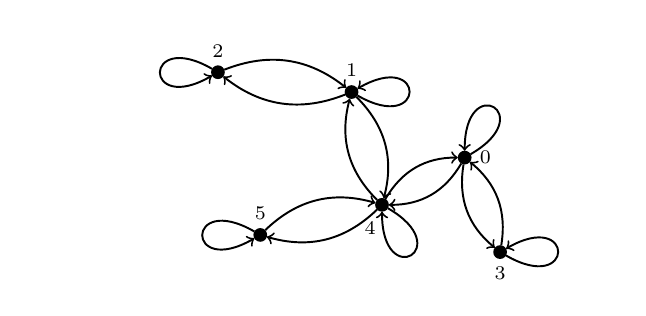
\begin{tikzpicture}[dot/.style={draw,circle,fill,inner sep=1.5pt},line width=.7pt,x=1.5cm,y=1.5cm]
\clip(-1,1.3) rectangle (4,3.5);
\begin{scriptsize}
\node[label=right:0] (r0) at (2.7,2.4) [dot] {};

\node[label=above:1] (r1) at (1.7420645075484014,2.9548225063123694) [dot] {};
%\draw[color=black] (1.8316581320147085,3.195605372065557) node {$1$};


\node[label=above:2] (r2) at (0.6109449986613309,3.1228105521866865) [dot] {};
%\draw[color=black] (0.7005386231276353,3.363593417939874) node {$2$};

\node[label=below:3] (r3) at (3,1.6) [dot] {};
%\draw[color=black] (2.6,1.2357448368651927) node {$3$};

\node (r4) at (2,2) [dot] {};
\draw[color=black] (1.9,1.8) node {$4$};

\node[label=above:5] (r5) at (0.9693194965265414,1.7453085760172875) [dot] {};
%\draw[color=black] (1,2) node {$5$};

\draw[->] (r0) to[out=30,in=90,looseness=30] (r0);
\draw[->] (r1) to[out=-30,in=30,looseness=30] (r1);
\draw[->] (r2) to[out=150,in=210,looseness=30] (r2);
\draw[->] (r3) to[out=-30,in=30,looseness=30] (r3);
\draw[->] (r4) to[out=-30,in=-90,looseness=30] (r4);
\draw[->] (r5) to[out=150,in=210,looseness=30] (r5);

\draw[->] (r0) to[bend left] (r4);
\draw[->] (r4) to[bend left] (r0);

\draw[->] (r0) to[bend right] (r3);
\draw[->] (r3) to[bend right] (r0);

\draw[->] (r5) to[bend left] (r4);
\draw[->] (r4) to[bend left] (r5);

\draw[->] (r1) to[bend left] (r4);
\draw[->] (r4) to[bend left] (r1);

\draw[->] (r1) to[bend left] (r2);
\draw[->] (r2) to[bend left] (r1);

\end{scriptsize}
\end{tikzpicture}
%\end{document}

\caption{Um exemplo de árvore e sua transformação como um digrafo a ser usado para sua representação por trilha Euleriana.}
\label{fig:exemploSeqEuler}
\end{figure}

A representação da árvore~$T$ é essencialmente a sequência de arcos que forma uma trilha Euleriana de~$T$.
Denotamos cada arco pelo par de vértices que o compõe.
\NEW{
Isto é, o arco que com origem no vértice~$u$ e destino no vértice~$v$ é escrito como $uv$.
Dessa forma, um laço em~$v$ é escrito como~$vv$.
Utilizaremos esses laços como representantes dos vértices na sequência. 
}
Por exemplo, a sequência~\eqref{eq:eulerSeq} representa a árvore da  Figura \ref{fig:exemploSeqEuler}.

\begin{equation}
30~00~04~41~12~22~21~11~14~44~45~55~54~40~03~33.\label{eq:eulerSeq}  
\end{equation}

Note que a sequência depende do vértice inicial e da ordem em que cada vizinho de cada vértice é visitado. Chamaremos uma tal sequência de \defi{sequência Euleriana} da árvore~$T$.

Henzinger e King \cite{HenzingerKing} propuseram armazenar uma sequência Euleriana em uma \defi[arvore@\'arvore!binária de busca]{árvore binária de busca} (ABB), que é uma árvore binária composta por nós que possuem  quatro campos: chave, pai, filho esquerdo e filho direito~\cite{CLRS}.

Os campos pai e filhos atribuem a estrutura de árvore binária à ABB. Isto é, cada nó~$N$ possui até dois filhos (esquerdo e direito), o campo \defi{pai} de cada um dos filhos aponta para~$N$. Nenhum nó é filho de dois outros nós. Pode ocorrer de um nó não possuir algum dos filhos; nesse caso, os campos correspondentes a filhos inexistentes contêm~$\Nil$. Somente um nó não possui pai: este é chamado de \defi{raiz} da ABB.

Para uma árvore binária ser considerada de busca, é necessário que, para todo nó $N$, todas as chaves da subárvore esquerda sejam menores do que a chave de $N$ e, simetricamente, todas as chaves da subárvore direita sejam maiores do que a chave de $N$.

Cada nó da ABB guarda um elemento da sequência Euleriana, ou seja, um par de vértices da árvore $T$, em um campo adicional \defi{info}\todo{o que acha de substituir o nome "info" por "arco"?}, e armazena, no campo \defi{chave}, \NEW{um valor entre $1$ e $n$ correspondente ao índice desse elemento na sequência, onde $n$ é o comprimento da sequência.}

\begin{figure}[htb]
%\scalebox{.6}{
\centering
\input{fig/SEQ-INDICES.tex}%}
\caption{Sequência~\eqref{eq:eulerSeq}  armazenada em uma ABB. Dentro do círculo mostramos o campo $info$ e abaixo do círculo está sua chave.}
\label{fig:seq-treap-indices}
\end{figure}
%\TODO{Perguntar ao Mota sobre o comentario dele, "Tem uns . no meio"

Por exemplo, a ABB na Figura~\ref{fig:seq-treap-indices} está armazenando a sequência Euleriana~\eqref{eq:eulerSeq}.
Uma tal ABB é chamada de \defi[arvore@\'arvore!Euleriana]{árvore Euleriana}. 
Henzinger e King propuseram representar uma floresta por uma coleção de Euler tour trees: uma para cada componente da floresta. 
Dessa forma, como veremos na Seção~\ref{sec:impleDF-ETT}, é possível obter uma implementação de uma floresta dinâmica em que as operações de consulta de conexidade e de inserção e remoção de aresta têm custo~$\O{\lg n}$, onde $n$ é o número de vértices da floresta.


\section{Implementação de floresta dinâmica com Euler tour trees}
\label{sec:impleDF-ETT}

\NEW{
Para implementar a biblioteca de florestas dinâmicas com Euler tour trees, consideremos inicialmente a seguinte biblioteca.
}

\begin{itemize}
\item  \treapCreate($u$, $v$): cria e retorna uma ABB com somente um nó que armazena o par de vértices $uv$;
\item \treapGetRoot($\node$): retorna a raiz da ABB que contém $\node$;
\item \treapJoin($T_1, T_2, \ldots, T_k$): junta as ABBs $T_1, T_2, \ldots, T_{k-1}$ e $T_k$ de modo que a sequência armazenada na árvore resultante é a concatenação das sequências armazenada em~$T_1, T_2, \ldots, T_k$ e retorna a raiz dessa árvore resultante.
\end{itemize}

A implementação dessas rotinas será detalhada no Capítulo~\ref{sec:TreapDeChaveImplicita}. Veremos que o consumo esperado de \treapCreate, \treapGetRoot{} e \treapJoin{} será, respectivamente,~$\O{1}$,~$\O{\lg n}$ e~$\O{h}$, onde~$n$ é o número de nós na ABB e~$h$ é a soma das alturas de~$T_1, T_2, \ldots, T_k$. Na Seção~\ref{sec:imple-treap}, mostraremos como implementar \treapJoin{} para o caso $k=2$, a extensão para o caso geral é imediato a partir desse caso particular.

\TODO{Remover ocorrência de hash e colocar dicionario ou tabela de símbolos}
Além disso, precisaremos também de uma tabela de símbolos para guardar, para cada par de vértices $uv$ da floresta, um apontador para um nó da ABB que contém esse par, ou $\Nil$ se um tal nó não existe. Quando $ u\neq v$, existe no máximo um nó nas ABBs com o par $uv$, porém para o par $uu$ podem existir vários nós na ABB da componente de $u$ na floresta. Para tal, usaremos um dicionário que guarda na $uv$-ésima posição um ponteiro para tal ocorrência de $uv$ ou $\Nil$, caso não haja ocorrência de $uv$. Para manusear a tabela, usaremos a seguinte biblioteca, que assumiremos que cada rotina dela consome tempo esperado~$\O{1}$~\cite{CLRS}.
\begin{itemize}
    \item $F~\gets~\hashCreate(n)$: cria e retorna uma tabela de símbolos $F$ capaz de armazenar os $n^2$ pares de vértices com uma informação~$valor$ associado;
    \item $F[u,v]~\gets~uv$: guarda o par $uv$ com valor associado~$uv$ na tabela~$F$. Se o par~$uv$ já estiver presente na tabela de símbolos, então seu valor associado é substituído por~$uv$;
    \item $F[u,v]~\gets~\Nil{}$: remove o conteúdo do par~$uv$ da tabela de símbolos;
    \item $var~\gets~F[u,v]$: atribui o valor associado ao par~$uv$ à variável $var$.
\end{itemize}

A ocorrência $uu$ apontada pela tabela de símbolos é chamada de \defi{ocorrência ativa} de~$u$.
No Algoritmo~\ref{Algo:dymForestCreate} apresentamos a implementação de~\dymForestCreate{}, que cria e retorna uma nova floresta dinâmica que possui $n$ vértices e nenhuma aresta.
Já no algoritmo~\ref{Algo:dymForestQuery}, mostramos a implementação de~\dymForestQuery{}, que responde a consulta de conexidade entre dois vértices~$u$ e~$v$ na floresta~$F$.


\begin{algorithm}[htb]
\caption{\dymForestCreate($n$)}
\label{Algo:dymForestCreate}
\begin{algorithmic}[1]
\State $F~\gets~\hashCreate(n^2)$
\For {$v$ $\gets$ 1 até $n$}\label{Algo:dymForestCreate:for}
\State $F[v,v]~\gets$ \treapCreate($v$, $v$)
\EndFor
\State \Return $F$
\end{algorithmic}
\end{algorithm}

Com essa implementação, em uma floresta com~$n$ vértices, \dymForestCreate{} consumirá tempo~$\O{n}$. A rotina \dymForestQuery{}, descrita no Algoritmo~\ref{Algo:dymForestQuery}, consumirá tempo esperado $\O{\lg n}$.


\begin{algorithm}[htb]
\caption{\dymForestQuery($F$, $u$, $v$)}
\label{Algo:dymForestQuery}
\begin{algorithmic}[1]
\State $uu$ $\gets$ $F[u,u]$
\State $vv$ $\gets$ $F[v,v]$
\State \Return \treapGetRoot($uu$) = \treapGetRoot($vv$)
\end{algorithmic}
\end{algorithm}

\TODO{Mota: "Justificar aqui a razão disso estar mais para frente pq alg 4 vem depois do 3?" Podemos explicar melhor ou trocar eles de lugar}
Para a operação \dymForestAddEdge{}, descrita no Algoritmo~\ref{Algo:dymForestAddEdge}, primeiro utilizamos a rotina auxiliar \ETmovetofront{}, descrita no Algoritmo~\ref{Algo:ETmovetofront}, que restrutura as ABBs que contém $uu$ e $vv$ de forma que estes se tornem os primeiros elementos de suas respectivas sequências Eulerianas. Por exemplo, se aplicarmos \ETmovetofront($T$,0), onde $T$ é a ABB que armazena a sequência~\eqref{eq:eulerSeq}, a ABB $T$ será reorganizada para armazenar a sequência:
\begin{equation}
00~04~44~41~11~12~22~21~11~14~44~45~55~54~44~43~33~34~44~40~00.\nonumber
\end{equation}

Após a aplicação de \ETmovetofront{}, utilizamos \treapJoin{} para juntar as ABBs com novas ocorrências de $uv$, $vu$ e~$uu$ na ordem apropriada para que a sequência resultante corresponda à sequência Euleriana da árvore obtida da adição da aresta~$uv$ à floresta.

\TODO{IMPORTANTE: Explicar, possivelmente com figuras, o funcionamento de cada algoritmo!!!!!!!!!}
\begin{algorithm}[htb]
\caption{\dymForestAddEdge($F$, $u$, $v$)}
\label{Algo:dymForestAddEdge}
\begin{algorithmic}[1]
\State \ETmovetofront($F$, $u$)
\State \ETmovetofront($F$, $v$)
\State $U$ $\gets$ \treapGetRoot($F[u,u]$)
\State $V$ $\gets$ \treapGetRoot($F[v,v]$)
\State $uv$ $\gets$ \treapCreate($u$, $v$)
\State $vu$ $\gets$ \treapCreate($v$, $u$)
\State $uu$ $\gets$ \treapCreate($u$, $u$)
\State $F[u,v]$ $\gets$ $uv$
\State $F[v,u]$ $\gets$ $vu$
\State \treapJoin($U$, $uv$, $V$, $vu$, $uu$)
\end{algorithmic}
\end{algorithm}
\begin{figure}[htb]
\centering
\begin{tikzpicture}[line cap=round,line join=round,>=triangle 45,x=1cm,y=1cm]
\clip(-.1,-.1) rectangle (11.1,1.1);
\draw [line width=1pt] (0,0)-- (1,0);
\draw [line width=1pt] (0,0)-- (0,1);
\draw [line width=1pt] (1,1)-- (1,0);
\draw [line width=1pt] (1,1)-- (1.5,1);
\draw [line width=1pt] (1,0)-- (1.5,0);
\draw [line width=1pt,dash pattern=on 1pt off 2pt] (1.5,0)-- (2.5,0);
\draw [line width=1pt,dash pattern=on 1pt off 2pt] (1.5,1)-- (2.5,1);
\draw [line width=1pt] (2.5,1)-- (3,1);
\draw [line width=1pt] (3,1)-- (3,0);
\draw [line width=1pt] (3,0)-- (2.5,0);
\draw [line width=1pt] (3,1)-- (4,1);
\draw [line width=1pt,color=ccqqqq] (4,1)-- (4,0);
\draw [line width=1pt] (4,0)-- (3,0);
\draw (.05,0.8) node[anchor=north west] {\Large $uu$};
\draw (1.05,0.8) node[anchor=north west] {\Large $u$};
\draw (2.45,0.8) node[anchor=north west] {\Large $u$};
\draw (3.05,0.8) node[anchor=north west] {\Large $uu$};
\draw [line width=1pt] (0,1)-- (1,1);
\draw [line width=1pt,color=ccqqqq] (4,0)-- (5,0);
\draw [line width=1pt,color=ccqqqq] (4,1)-- (5,1);
\draw [line width=1pt,color=ccqqqq] (5,1)-- (5,0);
\draw [line width=1pt] (6,0)-- (6,1);
\draw [line width=1pt] (6,0)-- (6.5,0);
\draw [line width=1pt] (6,1)-- (6.5,1);
\draw [line width=1pt,dash pattern=on 1pt off 2pt] (6.5,0)-- (7.5,0);
\draw [line width=1pt,dash pattern=on 1pt off 2pt] (6.5,1)-- (7.5,1);
\draw [line width=1pt] (7.5,0)-- (8,0);
\draw [line width=1pt] (7.5,1)-- (8,1);
\draw [line width=1pt] (8,1)-- (8,0);
\draw [line width=1pt] (8,0)-- (9.006976519904743,0);
\draw [line width=1pt] (8,1)-- (9,1);
\draw [line width=1pt,color=ccqqqq] (9.006976519904743,0)-- (9,1);
\draw [line width=1pt] (5,0)-- (6,0);
\draw [line width=1pt] (5,1)-- (6,1);
\draw (5.05,0.8) node[anchor=north west] {\Large $vv$};
\draw (6.05,0.8) node[anchor=north west] {\Large $v$};
\draw (7.45,0.8) node[anchor=north west] {\Large $v$};
\draw (8.05,0.8) node[anchor=north west] {\Large $vv$};
\draw [line width=1pt,color=ccqqqq] (9,1)-- (10,1);
\draw [line width=1pt,color=ccqqqq] (10,1)-- (10,0);
\draw [line width=1pt,color=ccqqqq] (10,0)-- (9.006976519904743,0);
\draw [line width=1pt,color=ccqqqq] (10,1)-- (11,1);
\draw [line width=1pt,color=ccqqqq] (11,1)-- (11,0);
\draw [line width=1pt,color=ccqqqq] (11,0)-- (10,0);
\draw (9.05,0.8) node[anchor=north west] {\red \Large $vu$};
\draw (10.05,0.8) node[anchor=north west] {\red \Large $uu$};
\draw (4.05,0.8) node[anchor=north west] {\red \Large $uv$};
\end{tikzpicture}
\caption{Sequência resultante de \dymForestAddEdge{}; blocos adicionais estão destacados em vermelho.}
\label{fig:algorit-link-seqxy}
\end{figure}


Veremos que o consumo de tempo esperado de \ETmovetofront{} é~$\O{\lg n}$, onde~$n$ é o número de nós na ABB. Consequentemente o consumo esperado de \dymForestAddEdge{} também será~$\O{\lg n}$.

A implementação de \ETmovetofront{}, assim como de \dymForestDelEdge{}, requer mais algumas rotinas da biblioteca que Euler Tour Trees dará suporte:

\begin{itemize}
\item \treapSearch($T$, $k$): retorna o nó com chave $k$ da árvore $T$;
\item \treapOrder($T$, $\node$): recebe um ponteiro para um nó da árvore $T$ e retorna a sua chave;
\item \treapSplit($T$, $\node$): recebe um ponteiro para um nó da árvore $T$ e retorna duas ABBs, a primeira contendo todos os nós de $T$ com chaves estritamente menores do que a chave de $\node$ e a segunda contendo os demais nós de $T$; e
\item \treapGetLast($T$): retorna o nó de maior chave na árvore~$T$.
\end{itemize}

Na Seção~\ref{sec:imple-treap}, mostraremos a implementação dessas rotinas que consomem~$\O{\lg n}$, onde~$n$ é número de nós em~$T$. Usando a biblioteca completa, as implementações de \ETmovetofront{} e \dymForestDelEdge{} são apresentadas nos Algoritmos~\ref{Algo:ETmovetofront} e~\ref{Algo:dymForestDelEdge}.

\begin{algorithm}[htb]
\caption{\ETmovetofront($F$, $u$)}
\label{Algo:ETmovetofront}
\begin{algorithmic}[1]
\State $uu$ $\gets$ $F[u,u]$
\State $T$ $\gets$ \treapGetRoot($uu$)
\State $vv$ $\gets$ \treapSearch($T$,1)
\If {$vv$ $\neq$ $uu$} \Comment{$uu$ já está no começo da sequência.}
\State $F[v,v]$ $\gets$ $vv$ \Comment{atualiza tabela de símbolos com uma ocorrência que não será apagada}.
\State $A$, $B$ $\gets$ \treapSplit($T$, $uu$)
\State $vv$ $\gets$ \treapGetLast($B$)
\State $B$, $C$ $\gets$ \treapSplit($T$, $vv$)\Comment{$C$ = $vv$}
\State $uu$ $\gets$ \treapCreate($u$, $u$)
\State \treapJoin($B$, $A$, $uu$)
\EndIf
\end{algorithmic}
\end{algorithm}

Na operação \dymForestDelEdge($F$, $uu$, $vv$), descrita no Algoritmo~\ref{Algo:dymForestDelEdge}, usamos a rotina \treapSplit{} para fatiar a ABB que guarda a sequência que contém $uv$ e $vu$ em cinco parte, nomeadas de $A$ a $E$, como ilustrado na Figura~\ref{fig:algorit-cut-seqxy}, que considera o caso em que $uv$ ocorre antes de $vu$ na sequência. Com essas cinco partes em mãos, descartaremos os trechos $B$ e $D$, e concatenamos as partes $A$ e $E$ para obter a sequência Euleriana das árvores resultantes da remoção de~$uv$. Como todas essas operações são feitas em tempo esperado~$\O{\lg n}$, então \dymForestDelEdge{} também possui consumo esperado de tempo~$\O{\lg n}$.

\begin{figure}[htb]
\centering
\definecolor{ccqqqq}{rgb}{1,0,0}
\definecolor{qqqqcc}{rgb}{0,0,1}
\begin{tikzpicture}[line cap=round,line join=round,>=triangle 45,x=1cm,y=1cm]
\clip(-.1,-.6) rectangle (10.1,1.1);
\draw (-.1,0.8) node[anchor=north west] {\Large $w$};
\draw [line width=1pt] (0,0)-- (3,0);
\draw [line width=1pt] (0,1)-- (3,1);

\draw [line width=1pt] (0,0)-- (0,1);
\draw (2.45,0.8) node[anchor=north west] {\Large $u$};
\draw [line width=1pt] (3,1)-- (3,0);
\draw (1.2,0.85) node[anchor=north west] {\Large $A$};


\draw (4.05,0.8) node[anchor=north west] {\Large $uv$};
\draw [line width=1pt] (4,0)-- (5,0);
\draw [line width=1pt] (4,1)-- (5,1);
\draw [line width=1pt] (5,1)-- (5,0);
\draw [line width=1pt] (4,1)-- (4,0);


\draw [line width=1pt] (6,0)-- (6,1);
\draw [line width=1pt] (6,0)-- (10,0);
\draw [line width=1pt] (6,1)-- (10,1);
\draw [line width=1pt] (10,1)-- (10,0);
\draw (9.3,0.8) node[anchor=north west] {\Large $w$};

\draw (6.05,0.8) node[anchor=north west] {\Large $v$};
\draw (7.5,0.85) node[anchor=north west] {\Large $B$};
\end{tikzpicture}

\caption{Sequência que será submetida ao \dymForestDelEdge{}; partes em vermelho serão descartadas.}
\label{fig:algorit-cut-seqxy}
\end{figure}

Como exemplo do funcionamento desses algoritmos, se removermos a aresta $41$ da árvore da Figura~\ref{fig:exemploSeqEuler}, obteremos as seguintes sequências:
\begin{equation}
00~04~{\red 44~41}~11~12~22~21~11~{\red 14}~44~45~55~54~44~43~33~34~44~40~00\nonumber
\end{equation}
\begin{equation}
11~12~22~21~11~~~~~~~~~~~~00~04~44~45~55~54~44~43~33~34~44~40~00.\label{eq:seqDel}
\end{equation}

Em seguida, para adicionar uma aresta ligando os vértices~2 e~5 da floresta~$F$ representada pelas sequências em~\eqref{eq:seqDel}, primeiro é aplicado \ETmovetofront($F$,2) e \ETmovetofront($F$,5) que resulta nas sequências:
\begin{equation}
22~21~11~12~22   ~~~~~~~~~~~~55~54~44~43~33~34~44~40~00~04~44~45~55.\nonumber
\end{equation}%{eq:bringToFront}
Em seguida, obteremos a seguinte sequência ao final de \ETTAddEdge($F$,2,5):
\begin{equation}
22~21~11~12~22~{\red 25}~55~54~44~43~33~34~44~40~00~04~44~45~55~{\red 52~22}.\nonumber
\end{equation}% \label{eq:seqAdd}

\begin{algorithm}[htb]
\caption{\dymForestDelEdge($F$, $u$, $v$)}
\label{Algo:dymForestDelEdge}
\begin{algorithmic}[1]
\State $Kuv$ $\gets$ \treapOrder($F[u,v]$)
\State $Kvu$ $\gets$ \treapOrder($F[v,u]$) 
\If {$Kuv$ $>$ $Kvu$}
	\Comment{garante que $uv$ aparece na sequência antes de $vu$}
	\State $u$ $\leftrightarrow$ $v$
	\State $Kuv$ $\leftrightarrow$ $Kvu$
\EndIf
\State $S$ $\gets$ \treapGetRoot($uv$)
\State $uu$ $\gets$ \treapSearch($S$, $Kuv-1$)\Comment{obtém a ocorrência de $uu$ que precede $uv$}
\State $vv$ $\gets$ \treapSearch($S$, $Kuv+1$)
\State $A$, $B$ $\gets$ \treapSplit($S$, $uu$)
\State $B$, $C$ $\gets$ \treapSplit($B$, $vv$)
\State $C$, $D$ $\gets$ \treapSplit($C$, $vu$)
\State $uu$ $\gets$ \treapSearch($D$, $2$)
\State $D$, $E$ $\gets$ \treapSplit($D$, $uu$)
\State $F[u,u]$ $\gets$ $uu$
\State $F[u,v]$ $\gets$ $\Nil{}$
\State $F[v,u]$ $\gets$ $\Nil{}$
\State \treapJoin($A$, $E$)
\end{algorithmic}
\end{algorithm}





